\documentclass[10pt]{article}

%%%%%%%%%%%%%%%%%%%%%%%%%%%%%%%%%%%%%%%%%%%%%%%%%%%%%%%%%%%%%%%%%%%%%%%%%%%%%%%%%%%%%%%%%%%%%%%%%%%%%%%%%%%%%%%%%%%%%
%%                                              LOAD PACKAGES
%%%%%%%%%%%%%%%%%%%%%%%%%%%%%%%%%%%%%%%%%%%%%%%%%%%%%%%%%%%%%%%%%%%%%%%%%%%%%%%%%%%%%%%%%%%%%%%%%%%%%%%%%%%%%%%%%%%%%
\usepackage{ifpdf}
\usepackage[load-configurations=abbreviations]{siunitx}     % define units
\usepackage{color}                                          % add colors to text (and highlight)
\usepackage{soul}                                           % for highlighting
\usepackage{amsmath}                                        % for mathematical formula
\usepackage{amssymb}                                        % mathematical symbols (might not be useful)
\usepackage{booktabs}                                       % for arrays: toprule, midrule, bottomrule
\usepackage{multirow}                                       % for arrays
\usepackage{graphicx}                                       % for \includegraphics
\usepackage{rotating}                                       % for sideways and other rotating stuffs
\usepackage{authblk}                                        % for authors and affiliations
\usepackage[printonlyused,withpage]{acronym}
%\usepackage[printonlyused,withpage,nohyperlinks]{acronym}


\ifpdf
    \usepackage[subrefformat=parens]{subcaption}                % for subfigures (replaces the subfig package:
                                                                % more up-to-date and works well with hyperref)
    \pdfoptionpdfminorversion=6                                 % Solves "found PDF version 1.6, but at most version
                                                                % 1.5 allowed" warning
\fi

\usepackage[
            backend         = biber
            , style         = authoryear-comp   %numeric-comp, authoryear-comp
            , sorting       = nyt               % name, title, year
            , maxbibnames   = 10                % maximum number of authors to mention in the bibliography, if reached,
            , minbibnames   = 1                 % the number of authors to cite is set to minbibnames (et al.)
            , maxcitenames  = 2                 % same for within the text (makes sense with only specific cite styles)
            , mincitenames  = 1
            , backref       = false             % indicate or not the page on which the bibliography item is cited
            , backrefstyle  = three
            , abbreviate    = true              % default (Volume -> Vol., pages -> pp., ...)
            , doi           = false
            , isbn          = false
            , url           = false
            , eprint        = false
            , firstinits    = true              % all first and middle names as initials
            , uniquename    = init              % Disambiguate names using initials only (to be compatible with firstinits = true)
            ]{biblatex}

%\addbibresource{d:/KULeuven/PhD/MendeleyBiblioAbbr.bib}
%\addbibresource{d:/KULeuven/PhD/Publish/JournalPublications/Neuroimage/draft/AdditionalBiblioAbbr.bib}
\addbibresource{d:/KULeuven/PhD/MendeleyBiblio.bib}
%\addbibresource{d:/KULeuven/PhD/Publish/JournalPublications/Neuroimage/draft/AdditionalBiblio.bib}

% TO LOAD LAST FOR COMMANDS NOT TO BE OVERWRITTEN
\usepackage[bookmarksopen,colorlinks,linkcolor=blue,citecolor=blue]{hyperref} % for \autoref and hyperlinks

%%%%%%%%%%%%%%%%%%%%%%%%%%%%%%%%%%%%%%%%%%%%%%%%%%%%%%%%%%%%%%%%%%%%%%%%%%%%%%%%%%%%%%%%%%%%%%%%%%%%%%%%%%%%%%%%%%%%%
%%                                           DOCUMENT OPTIONS
%%%%%%%%%%%%%%%%%%%%%%%%%%%%%%%%%%%%%%%%%%%%%%%%%%%%%%%%%%%%%%%%%%%%%%%%%%%%%%%%%%%%%%%%%%%%%%%%%%%%%%%%%%%%%%%%%%%%%

%--------------------------------------------------
% biblatex options
%--------------------------------------------------

%% remove "in:" from articles
%\renewbibmacro*{in:}{%
%  \ifentrytype{article}{}{%
%    \printtext{%
%      \bibstring{in}\intitlepunct}}}

%\renewcommand{\newunitpunct}{}
%\renewcommand{\newblockpunct}{}

% remove "in" before journal/conference/... title
\renewbibmacro*{in:}{}

% remove "month" from all entries
\AtEveryBibitem{%
  \clearfield{month}%
}

% in bibliography: last name, first name
\DeclareNameAlias{sortname}{last-first}

% remove quote for title (remove italic for book title) (check original in biblatex.def)
\DeclareFieldFormat
  [article,inbook,incollection,inproceedings,patent,thesis,unpublished,book]
  {title}{#1\isdot}

% remove pp. for pages
\DeclareFieldFormat
  [article,inbook,incollection,inproceedings]
  {pages}{#1}

% remove italic for journal/collection/proceeding title
\DeclareFieldFormat{journaltitle}{#1}
\DeclareFieldFormat{booktitle}{{#1}}

% remove parenthesis from year
\makeatletter
\def\act@on@bibmacro#1#2{%
  \expandafter#1\csname abx@macro@\detokenize{#2}\endcsname
}
\def\patchbibmacro{\act@on@bibmacro\patchcmd}
\def\pretobibmacro{\act@on@bibmacro\pretocmd}
\def\apptobibmacro{\act@on@bibmacro\apptocmd}
\def\showbibmacro{\act@on@bibmacro\show}
\makeatother

\patchbibmacro{date+extrayear}{%
  \printtext[parens]%
}{%
  \addcomma\space%
  \printtext%
}{}{}

% volume (number) formatting
\newbibmacro*{volume+number+eid}{%
  \printfield{volume}%
  %\space%
  \iffieldundef{number}{}{
  \printtext[parens]{%
  \printfield{number}}%
  \setunit{\addcomma\space}%
  \printfield{eid}}}

% Citation Hyperlinks (not just years), thanks to Audrey.
\makeatletter
\renewbibmacro*{cite}{% Based on cite bib macro from authoryear-comp.cbx
  \iffieldundef{shorthand}
    {\ifthenelse{\ifnameundef{labelname}\OR\iffieldundef{labelyear}}
       {\printtext[bibhyperref]{% Include labelname in hyperlink
          \DeclareFieldAlias{bibhyperref}{default}% Prevent nested hyperlinks
          \usebibmacro{cite:label}%
          \setunit{\addspace}%
          \usebibmacro{cite:labelyear+extrayear}}%
          \usebibmacro{cite:reinit}}
       {\iffieldequals{namehash}{\cbx@lasthash}
          {\ifthenelse{\iffieldequals{labelyear}{\cbx@lastyear}\AND
                       \(\value{multicitecount}=0\OR\iffieldundef{postnote}\)}
             {\setunit{\addcomma}%
              \usebibmacro{cite:extrayear}}
             {\setunit{\compcitedelim}%
              \usebibmacro{cite:labelyear+extrayear}%
              \savefield{labelyear}{\cbx@lastyear}}}
          {\printtext[bibhyperref]{% Include labelname in hyperlink
             \DeclareFieldAlias{bibhyperref}{default}% Prevent nested hyperlinks
             \printnames{labelname}%
             \setunit{\nameyeardelim}%
             \usebibmacro{cite:labelyear+extrayear}}%
             \savefield{namehash}{\cbx@lasthash}%
             \savefield{labelyear}{\cbx@lastyear}}}}
    {\usebibmacro{cite:shorthand}%
     \usebibmacro{cite:reinit}}%
  \setunit{\multicitedelim}}

\renewbibmacro*{textcite}{% Based on textcite bib macro from authoryear-comp.cbx
  \iffieldequals{namehash}{\cbx@lasthash}
    {\iffieldundef{shorthand}
       {\ifthenelse{\iffieldequals{labelyear}{\cbx@lastyear}\AND
                    \(\value{multicitecount}=0\OR\iffieldundef{postnote}\)}
          {\setunit{\addcomma}%
           \usebibmacro{cite:extrayear}}
          {\setunit{\compcitedelim}%
           \usebibmacro{cite:labelyear+extrayear}%
           \savefield{labelyear}{\cbx@lastyear}}}
       {\setunit{\compcitedelim}%
        \usebibmacro{cite:shorthand}%
        \global\undef\cbx@lastyear}}
    {\ifnameundef{labelname}
       {\printtext[bibhyperref]{% Include labelname in hyperlink
          \DeclareFieldAlias{bibhyperref}{default}% Prevent nested hyperlinks
          \iffieldundef{shorthand}
            {\usebibmacro{cite:label}%
             \setunit{%
               \global\booltrue{cbx:parens}%
               \addspace\bibopenparen}%
             \ifnumequal{\value{citecount}}{1}
               {\usebibmacro{prenote}}
               {}%
             \usebibmacro{cite:labelyear+extrayear}}
            {\usebibmacro{cite:shorthand}}%
          \ifthenelse{\iffieldundef{postnote}\AND
                      \(\value{multicitetotal}=0\AND\value{citetotal}=1\)}
            {\bibcloseparen% Include closing parenthesis in hyperlink
             \global\boolfalse{cbx:parens}}
            {}}}
       {\printtext[bibhyperref]{% Include labelname in hyperlink
          \DeclareFieldAlias{bibhyperref}{default}% Prevent nested hyperlinks
          \printnames{labelname}%
          \setunit{%
            \global\booltrue{cbx:parens}%
            \addspace\bibopenparen}%
          \ifnumequal{\value{citecount}}{1}
            {\usebibmacro{prenote}}
            {}%
          \iffieldundef{shorthand}
            {\iffieldundef{labelyear}
               {\usebibmacro{cite:label}}
               {\usebibmacro{cite:labelyear+extrayear}}%
             \savefield{labelyear}{\cbx@lastyear}}
            {\usebibmacro{cite:shorthand}%
             \global\undef\cbx@lastyear}%
          \ifthenelse{\iffieldundef{postnote}\AND
                      \(\value{multicitetotal}=0\AND\value{citetotal}=1\)}
            {\bibcloseparen% Include closing parenthesis in hyperlink
             \global\boolfalse{cbx:parens}}
            {}}%
          \savefield{namehash}{\cbx@lasthash}}}%
  \setunit{%
    \ifbool{cbx:parens}
      {\bibcloseparen\global\boolfalse{cbx:parens}}
      {}%
    \multicitedelim}}

\makeatother



%--------------------------------------------------
% Define highlight color
%--------------------------------------------------
\definecolor{hlColor}{RGB}{255, 255, 102}
\sethlcolor{hlColor}

%--------------------------------------------------
% superscripts
%--------------------------------------------------
\newcommand{\superscript}[1]{\ensuremath{^{\textrm{#1}}}}
\newcommand{\nth}[0]{\superscript{th} }
\newcommand{\rd}[0]{\superscript{rd} }
%\newcommand{\st}[0]{\superscript{st}}

%--------------------------------------------------
% autoref names for hyperref package
%--------------------------------------------------
\def\figureautorefname{Fig.}
\def\sectionautorefname{sec.}
\def\subsectionautorefname{sec.}
\def\subsubsectionautorefname{sec.}
\def\equationautorefname{eq.}


%--------------------------------------------------
% line space: 1.3->1.5, 1.6->2
%--------------------------------------------------
%\linespread{1.6}

\ifpdf
    %--------------------------------------------------
    % page layout
    %--------------------------------------------------
    \addtolength{\topmargin}{-2cm}
    \addtolength{\textheight}{3cm}
    \addtolength{\evensidemargin}{-1.5cm}
    \addtolength{\oddsidemargin}{-1.5cm}
    \addtolength{\textwidth}{3cm}
\else
    %--------------------------------------------------
    %
    %--------------------------------------------------
    \makeatletter
    \newcommand\blx@unitmark{23sp}
    \makeatother
\fi



\acrodef{SSVEP}{Steady-State Visually Evoked Potential}
\acrodef{BCI}{Brain-Computer Interface}

%%%%%%%%%%%%%%%%%%%%%%%%%%%%%%%%%%%%%%%%%%%%%%%%%%%%%%%%%%%%%%%%%%%%%%%%%%%%%%%%%%%%%%%%%%%%%%%%%%%%%%%%%%%%%%%%%%%%%
%%%%%%%%%%%%%%%%%%%%%%%%%%%%%%%%%%%%%%%%%%%%%%%%%%%%%%%%%%%%%%%%%%%%%%%%%%%%%%%%%%%%%%%%%%%%%%%%%%%%%%%%%%%%%%%%%%%%%
%%%%%%%%%%%%%%%%%%%%%%%%%%%%%%%%%%%%%%%%%%%%%%%%%%%%%%%%%%%%%%%%%%%%%%%%%%%%%%%%%%%%%%%%%%%%%%%%%%%%%%%%%%%%%%%%%%%%%
%%%%%%%%%%%%%%%%%%%%%%%%%%%%%%%%%%%%%%%%%%%%%%%%%%%%%%%%%%%%%%%%%%%%%%%%%%%%%%%%%%%%%%%%%%%%%%%%%%%%%%%%%%%%%%%%%%%%%

\title{Hybrid oddball - SSVEP BCI}

\author[ * ]{A. Combaz}
\affil[ * ]{Computational Neuroscience Group, Laboratory for Neuro- and Psychophysiology, KU Leuven, Leuven, Belgium}

\renewcommand\Authands{ and } % remove the comma before "and"

\begin{document}


%%%%%%%%%%%%%%%%%%%%%%%%%%%%%%%%%%%%%%%%%%%%%%%%%%%%%%%%%%%%%%%%%%%%%%%%%%%%%%%%%%%%%%%%%%%%%%%%%%%%%%%%%%%%%%%%%%%%%
%%                                           FRONTMATTER
%%%%%%%%%%%%%%%%%%%%%%%%%%%%%%%%%%%%%%%%%%%%%%%%%%%%%%%%%%%%%%%%%%%%%%%%%%%%%%%%%%%%%%%%%%%%%%%%%%%%%%%%%%%%%%%%%%%%%
\maketitle

\begin{abstract}
Objectives:
blablabla blalabbla \ac{SSVEP}-based BCIs.

Results:
blablabla blablabla \ac{SSVEP} responses.

Conclusion:
\end{abstract}

%%%%%%%%%%%%%%%%%%%%%%%%%%%%%%%%%%%%%%%%%%%%%%%%%%%%%%%%%%%%%%%%%%%%%%%%%%%%%%%%%%%%%%%%%%%%%%%%%%%%%%%%%%%%%%%%%%%%%
%%                                           MAIN TEXT
%%%%%%%%%%%%%%%%%%%%%%%%%%%%%%%%%%%%%%%%%%%%%%%%%%%%%%%%%%%%%%%%%%%%%%%%%%%%%%%%%%%%%%%%%%%%%%%%%%%%%%%%%%%%%%%%%%%%%

\acresetall

%===================================================================================================================
%                                             1 INTRODUCTION
%===================================================================================================================
\section{Introduction}
\label{sec:1Intro}

% General BCI

% P3 BCI, definition, plus and minus

% SSVEP BCI, definition, plus and minus

% Hybrid BCI: definition

% Hybrid BCI: general examples

% Hybrid BCI: P3/SSVEP examples

% Hybrid BCI: what has not been done

% What we do here

%===================================================================================================================
%                                             2 MATERIALS AND METHODS
%===================================================================================================================
\section{Materials and Methods}
\label{sec:2MatAndMet}

    \subsection{Material}
    \label{sec:2.1Material}

    % EEG acq
    The EEG signals were recorded using a BioSemi Active Two system with 32~channels (following the 10-20 international system) at a sampling rate of \SI{1024}{\Hz}.
    Two additional electrodes were positioned on the right and left mastoids and the mean of the signals recorded at those two sites was used to reference the activity measured by the 32~EEG electrodes.

    % Stimuli presentation
    All stimulation employed MATLAB\textsuperscript{\textregistered}, the stimuli were visually presented on a laptop's LCD screen (\SI{60}{\Hz} refresh rate) and their display and timing used the \emph{Psychophysics Toolbox Extensions} (\cite{Brainard1997,Pelli1997}).



    \subsection{Experiment 1: studying the oddball ERPs}
    \label{sec:2.2Oddball}

        \subsubsection{Experimental protocol}
        \label{sec:2.2.1Protocol}

        % Aim and subjects
        The aim of this first experiment was to study the effect of a flickering background on the typical ERP response associated to an oddball paradigm.
        N subjects participated in the experiment (age, gender).

        % exp description
        As shown in \autoref{fig:stimSeq}, a typical \emph{stimulation cycle}, started with a \SI{2000}{\ms} cue, indicating the participant his/her target item, followed by a \SI{1000}{\ms} pause during which the cue disappears and all icons remained gray.
        The background rectangle then started to flicker and the oddball stimulation started \SI{500}{\ms} later.
        The oddball stimulation consisted of 10~\emph{flashing sequences} during which each of the 6~icons was flashed one after another in random order for a duration randomly set between \SIlist[list-units = single]{200;300}{\ms}.
        As usually done for oddball experiments, the participants were instructed to focus on their target symbol and count the number of time it flashes.
        A \SI{1000}{\ms} pause followed the oddball stimulation and preceded the next cue.
        An \emph{experimental run} lasted approximately 4~minutes and consisted of 12 consecutive stimulation cycles, so that each of the 6~icons was cued twice (in random order).

        As we aimed here at studying the effect of the flickering background on the oddball ERP response, we defined 5~experimental conditions.
        The first one (baseline) consisted of a run as described in the previous paragraph but in which no flickering background was displayed.
        The 4~other conditions differed only by the frequency of the flickering background; the frequencies used were \SIlist[list-units = single]{8.57;10;12;15}{\Hz}, corresponding to the division of the refreshing rate of the screen by \numlist{7;6;5;4}, respectively.

        For each of the 5~conditions, all subjects performed 3~runs, therefore the whole experiment consisted of 15~runs of approximately 4~minutes each.
        The order of the run was randomized for each subject and a 5~to~10~minutes pause was set up every 5~runs.

        % use
        The data collected were used to compare the shape of the oddball response (response to the flashing of the target icon) and the ERP classification accuracy (response to target \emph{v.s.} response to non-target flasing) across conditions.

        \subsubsection{Data Analysis: ERP responses}
        \label{sec:2.2.2AnalysisErpShape}

        % preprocessing: filtering

        % studying the shape of ERP: epoch rejection

        \subsubsection{Data Analysis: ERP classification}
        \label{sec:2.2.3AnalysisErpClassification}

        % studying classification accuracy: no epoch rejection


    \subsection{Experiment 2: studying the \acs{SSVEP} responses}
    \label{sec:2.3SSVEP}

        \subsubsection{Experimental protocol}
        \label{sec:2.3.1Protocol}

        % Aim and subjects
        The aim of this second experiment was to study the effect of an oddball paradigm on the \ac{SSVEP} responses.
        N subjects participated in the experiment (age, gender).

        % exp description
        The experimental run was the same as described in \autoref{sec:2.2.1Protocol}.
        Two experimental parameters were manipulated, the first one was the stimulation frequency; the same frequencies as for the first experiment were used (\SIlist[list-units = single]{8.57;10;12;15}{\Hz}).
        The second experimental parameter was the presence or not of the oddball stimulation sequence.
        When the oddball stimulation was displayed, the participants were instructed to count the number of flashes of the target icon, while when no oddball stimulation was displayed, their task was simply to focus on their target icon.
        
        The experiment consisted thus of 8~runs of approximately 4~minutes each.
        The order of the run was randomized for each subject and a 5~to~10~minutes pause was set up after the first 4~runs.

        % use
        This experimental design allows a comparison of the \ac{SSVEP} responses of the participants with and without an oddball stimulation superimposed on the \ac{SSVEP} stimulation for a different set of \ac{SSVEP} frequencies.


        \subsubsection{Data Analysis}
        \label{sec:2.3.2Analysis}
        
        % pre-processing
        
        % snr calculation
        
        % statistics


    \subsection{Experiment 3: hybrid classification}
    \label{sec:2.4Hybrid}

        \subsubsection{Experimental protocol}
        \label{sec:2.4.1Protocol}

        \subsubsection{Data Analysis}
        \label{sec:2.4.2Analysis}

%===================================================================================================================
%                                             3 RESULTS
%===================================================================================================================
\section{Results}
\label{sec:3Results}

    \subsection{Experiment 1: studying the oddball ERPs}
    \label{sec:2.2Oddball}


    \subsection{Experiment 2: studying the \ac{SSVEP} responses}
    \label{sec:2.3SSVEP}


    \subsection{Experiment 3: hybrid classification}
    \label{sec:2.4Hybrid}


%===================================================================================================================
%                                             4 DISCUSSION
%===================================================================================================================
\section{Discussion}
\label{sec:4Discuss}

%===================================================================================================================
%                                             5 CONCLUSION
%===================================================================================================================
\section{Conclusion}
\label{sec:6Conclusion}

%===================================================================================================================
%                                             5 ACKNOWLEDGMENTS
%===================================================================================================================
\section*{Acknowledgments}

\printbibliography

%%===================================================================================================================
%                                             TABLES
%===================================================================================================================


%===================================================================================================================
%                                             FIGURES
%===================================================================================================================
\clearpage

%-------------------------------------------------------------------------------------------------------------------
% oddball pix
%-------------------------------------------------------------------------------------------------------------------
\begin{figure}[t]
\centering
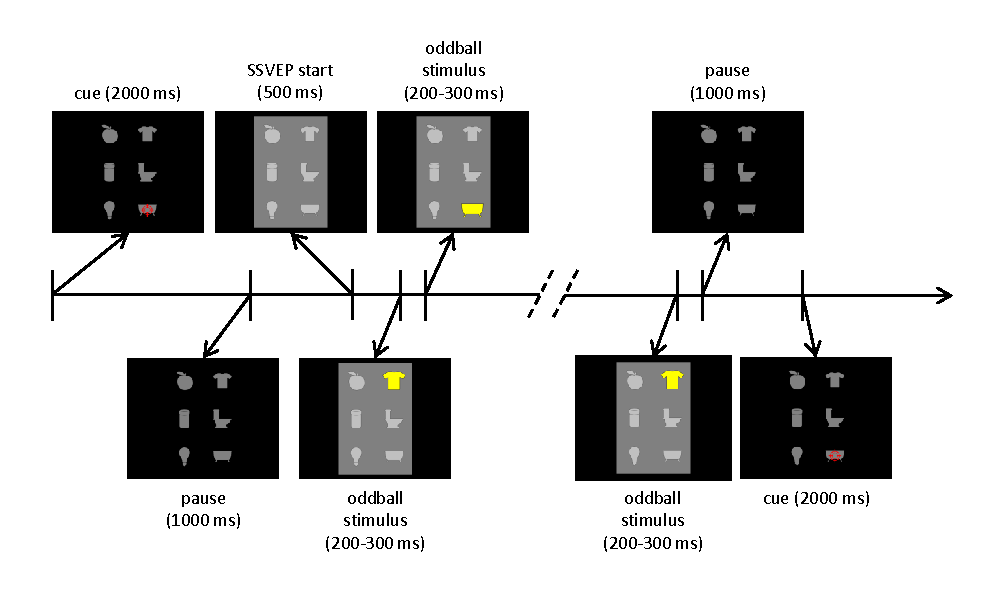
\includegraphics{pix/stimulationSequence}
\caption{stimulation sequence}
\label{fig:stimSeq}
\end{figure}

%===================================================================================================================
%                                             TABLES
%===================================================================================================================


%===================================================================================================================
%                                             FIGURES
%===================================================================================================================
\clearpage

%-------------------------------------------------------------------------------------------------------------------
% oddball pix
%-------------------------------------------------------------------------------------------------------------------
\begin{figure}[t]
\centering
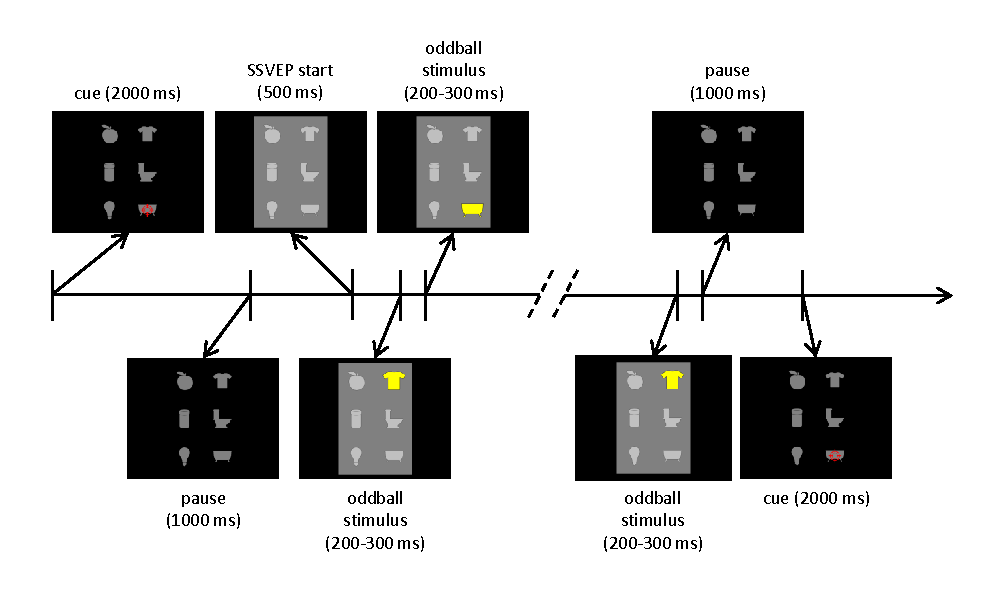
\includegraphics{pix/stimulationSequence}
\caption{stimulation sequence}
\label{fig:stimSeq}
\end{figure}

%\section{Acronyms}
%\begin{acronym}
%    \acro{SSVEP}{Steady-State Visually Evoked Potential}
%\end{acronym}

\end{document}
